%!TEX root = ../dokumentation.tex

\chapter{Konzept und Design}

Zum Projektstart wurde sich zunächst mit der Konzeption des genauen Anwendungsfalles und der benötigten Funktionen beschäftigt.
So konnte ein gemeinsames Verständnis für das Projekt entwickelt werden.
\\
Angedacht ist die Entwicklung einer Peer-to-Peer Bezahl-Applikation, mit der Anwender untereinander durch das Scannen eines individuellen QR-Codes Transaktionen durchführen können.
Der QR-Code sollte dafür entsprechend kodiert werden und den Zahlungsempfänger beinhalten, wohingegen der Betrag durch den Zahlungssender wählbar und durch ein numerisches Eingabefeld bestimmbar wäre.
\\
Im weiteren Verlauf wurde daran gearbeitet, nicht nur die Applikation technisch zu implementieren, sondern auch ansprechend gestalterisch umzusetzen. Um der App ebenfalls einen Namen und ein Gesicht zu geben, konnte mit wenig Aufwand ein Name gefunden und ein Logo generiert werden.
\\
Anschließend wurden noch Screendesigns angefertigt, an denen sich während der Umsetzung orientiert wurde. 

\section{Markenentwicklung}

Für das Projekt sollte ein passender Name gefunden werden, der den Bezug zur Kernfunktion, dem Bezahlen von Geldbeträgen widerspiegelt.
Um möglichst wenig Konfliktpotential zu bestehenden Unternehmen oder Institutionen zu bieten, wurde bei der Wahl des Namens im Oktober 2023 darauf geachtet, dass dieser möglichst keine Treffer bei der Suche mit Suchmaschinen wie Google bietet und auch der Name mit gängigen Top-Level-Domains noch verfügbar ist.  
\\
Mithilfe des KI-gestützten Tools Bing Chat, welches auf dem von OpenAI entwickeltem GPT-4 basiert, wurden dann Vorschläge entwickelt und anschließend durch die Autoren ausgewertet.
\\
Es wurde sich für den Namen „Payero“ entschieden, da die ersten Silben in vielen Sprachen mit dem Verb „bezahlen“ konnotieren.
So gibt es etwa im Französichen das Verb „payer“ und im Englisch das Nomen „payer“.
\\
Für das Logo wurden ebenfalls Vorschläge mit Bing Chat gesammelt, die dann als Grundlage genutzt und mit Grafiktools aufgearbeitet wurden.
Das Logo wurde um einen Schriftzug in der Schriftart Nunito ergänzt.
In Abbildung \ref{branding} wird das Logo alleinstehend auf hellem und dunklem Untergrund dargestellt, sowie die Kombination mit Schriftzug.

\begin{figure}[H]
  \centering
  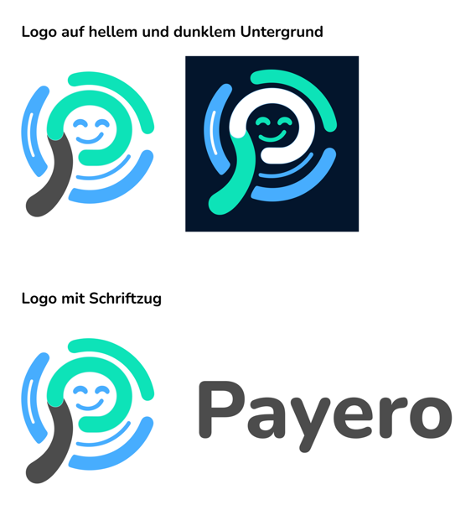
\includegraphics[width=0.8\textwidth]{images/branding.png}
  \caption{Darstellung des Logos auf hellen und dunklen Hintergründen, sowie in Kombination mit Schriftzug.}
  \label{branding}
\end{figure}

  \section{Wireframes}

  Das Konzept der Applikation sieht es vor, den Anwender durch mehrere Ansichten zu führen, bei denen unter anderem die Bezahlfunktionen umgesetzt, aber auch beispielsweise eine Transkations-Historie ausgegeben wird.
  Konkret sind folgende Ansichten angedacht:

  \subsubsection*{SplashScreen: Bildschirm mit kurzer Anzeigedauer beim Start der App}
  Der SplashScreen sollte beim Öffnen der App für einige Sekunden angezeigt werden und das Logo in Kombination mit dem Namen der App darstellen.
  Aus technischer Sicht könnten im Hintergrund bereits Daten geladen werden.
  \subsubsection*{MainScreen: Bildschirm mit Übersicht über letzte Transaktionen und Absprüngen zu den Kernfunktionen}
  Dieser Bildschirm stellt das zentrale Bedienfeld der App dar, da hier alle wichtigen Funktionen gebündelt werden.
  Es soll ein anklickbares Icon zum Absprung zum SettingsScreen dargestellt werden.
  Ebenso wird hier der persönliche und dynamisch generierte QR-Code präsentiert.
  Falls ein Benutzer seinen QR-Code an weitere Personen weitergeben möchte, kann er auf diesen bereits recht schnell nach dem Start der App zugreifen.
  Ein weiteres wichtiges Element dieses Bildschirms wird die Transakations-Historie sein, da hier der Endanwender auf den ersten Blick die zuletzt durchgeführten Transaktionen einsehen kann.
  Um zielgerichtet auf die Kernfunktion der App, dem Einscannen von QR-Codes anderer Teilnehmer, zu verweisen, wird hier ein großer Button mit dem Text „Scannen“ angedacht.
  Ein Klick auf diesen wird auf den QRScanScreen umleiten.
  \subsubsection*{SettingsScreen: Bildschirm mit Einstellungen und technischen Informationen zur App}
  Der SettingsScreen wird die Versionsnummer der App darstellen, sowie Informationen zu den Herausgebern. Sinnvoll wäre es hier ebenfalls einen Changelog unterzubringen und beispielsweise Einstellmöglichkeiten für Sprachwahl, oder ähnliche Benutzereinstellungen anzubieten. Für das Projekt wäre es ebenfalls denkbar hier Debug-Informationen wie etwa Benutzer-ID darzustellen.
  \subsubsection*{QRScanScreen: Bildschirm zum Erfassen von QR-Codes}
  Der QRScanScreen wird die zentrale Funktion bieten, die individuellen QR-Codes von anderen App-Nutzern einzuscannen.
  Sofern ein valider QR-Code erfasst wird, sollte auf den FoundCodeScreen umgeleitet werden.
  \subsubsection*{FoundCodeScreen: Bildschirm zur Tätigung der Transkation}
  Der FoundCodeScreen wird angezeigt, wenn ein valider QR-Code gescannt wurde und ein Zahlungsvorgang initiert werden kann.
  Für die Implementierung der Zahlungsabwicklung wird der Bezahldienstleister Braintree vorgesehen, der unter anderem Zahlungen mit PayPal, Kreditkarte, Google Pay und Apple Pay ermöglicht.
  Ein entsprechendes Widget soll hierfür an dieser Stelle eingebunden werden.
  \subsubsection*{EndScreen: Bildschirm zur Darstellung einer Erfolgsmeldung bei getätigter Transaktion}
  Nach erfolgreicher Zahlungsabwicklung sollte der Benutzer der App ein Feedback erhalten und wird daher zu einem EndScreen weitergeleitet.
  Hier werden noch einmal die wichtigsten Eckdaten zur kürzlich abgeschlossenen Transaktion dargestellt.
  Denkbar wäre es hier ebenfalls eine zum Design passende Illustration darzustellen, um den Endnutzer möglicherweise für die Tätigung weiterer Transaktionen zu animieren und den sonst langweiligen und tristen Bezahlprozess etwas aufzulockern.
  \\
  In Abbildung \ref{fig:wireframes} werden noch einmal gesammelt die angefertigten Entwürfe dargestellt.
  
  \begin{figure}[H]
    \centering
    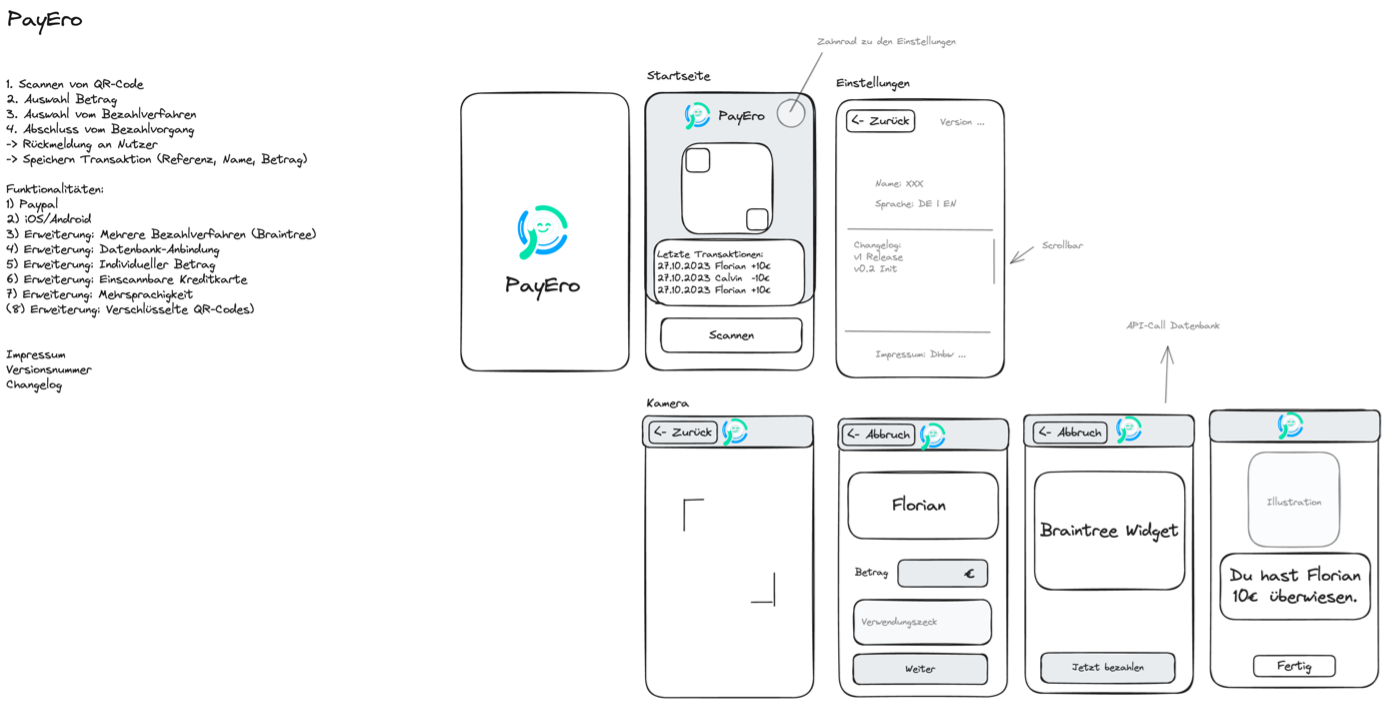
\includegraphics[width=0.8\textwidth]{images/wireframes.png}
    \caption{Darstellung der angefertigten Wireframes.}
    \label{wireframes}
  \end{figure}